\documentclass[12pt]{report}
\usepackage[T1]{fontenc}
\usepackage[utf8]{inputenc}
\usepackage[italian]{babel}
\usepackage{amsmath}
\usepackage{amssymb}
\usepackage{graphicx}
\usepackage{listings}
\usepackage{xcolor}
\usepackage{titling}
\usepackage{listings}
\usepackage[a4paper,left=2cm,right=2cm]{geometry}

\definecolor{codegreen}{rgb}{0,0.6,0}
\definecolor{codegray}{rgb}{0.5,0.5,0.5}
\definecolor{codepurple}{rgb}{0.58,0,0.82}
\definecolor{backcolour}{rgb}{0.95,0.95,0.92}

\lstdefinestyle{mystyle}{
	backgroundcolor=\color{backcolour},   
	commentstyle=\color{codegreen},
	keywordstyle=\color{magenta},
	numberstyle=\tiny\color{codegray},
	stringstyle=\color{codepurple},
	basicstyle=\ttfamily\footnotesize,
	breakatwhitespace=false,         
	breaklines=true,                 
	captionpos=b,                    
	keepspaces=true,                 
	numbers=left,                    
	numbersep=5pt,                  
	showspaces=false,                
	showstringspaces=false,
	showtabs=false,                  
	tabsize=2
}

\lstset{style=mystyle}

\begin{document}
	\author{Luca Fumagalli, Lorenzo D'Alessandro}
	\title{Relazione progetto \textit{Gestione dell’informazione geospaziale} }
	\date{\vspace{-5ex}}
	\maketitle

\chapter*{Rilevamento traiettoria}
Per rilevare la traiettoria usta all'interno del progetto abbiamo utilizzato l'applicazione Android \textit{Geo Tracker - GPS tracker}%
\footnote{https://play.google.com/store/apps/details?id=com.ilyabogdanovich.geotracker\&hl=it}.

Le geometrie delle strade sono state esportate dal sito di \textit{OpenStreetMap}.%
\footnote{https://www.openstreetmap.org/}

Il risultato dell'acquisizione della traiettoria e la sovrapposizione alla mappa è visibile in figura \ref{punto1}.
\begin{figure}
	\centering
	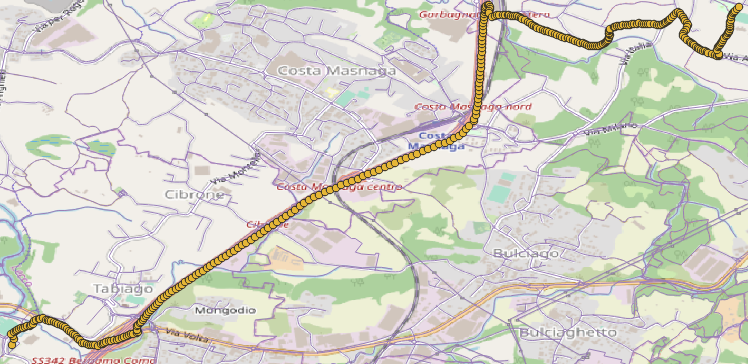
\includegraphics[scale = 0.55]{figures/punto1}
	\caption{Immagine presa da QGIS della mappa e della traiettoria}\label{punto1}
\end{figure}
\chapter*{Map Matching}
Per effettuare il \textit{map matching} abbiamo effettuato diverse operazioni:
\begin{itemize}
	\item Come prima operazione abbiamo dovuto prendere tutti i dati del tragitto dal database ed inserirli in una lista, ogni punto è rappresentato da una tupla i cui elementi sono le colonne della tabella \textit{tragitto} del database. \lstinputlisting[language=SQL]{code/query1.sql}
	\item Per ogni punto del tragitto cerchiamo la \textit{linestring} corrispondente alla strada più vicina. Per ogni punto creiamo una tupla formata dall'\textit{id} del punto e l'\textit{id} della strada più vicina che viene inserita nella lista \textit{point\_closest\_line\_list} \lstinputlisting[language=SQL]{code/query.sql}\lstinputlisting[language=Python]{code/python.py}
	\item Viene effettuato il \textit{fix} sui punti che si trovano isolati su una strada. \lstinputlisting[language=Python]{code/fix.py}
	\item Viene proiettato il punto sulla strada più vicina e viene inserito nel database nella tabella \textit{matched\_point}.
	\lstinputlisting[language=SQL]{code/match.sql}\lstinputlisting[language=Python]{code/matched.py}
\end{itemize}
	
\chapter*{Velocità}
	
	
	
	
	
	
	
	
\end{document}